\documentclass[11pt,  oneside, openany]{book}
\usepackage[greek, italian]{babel}
\usepackage{geometry}
\usepackage{float}
\usepackage{graphicx} 
\usepackage{amsmath}
\usepackage{array}
\usepackage{amsfonts}
\usepackage{multirow}
\geometry{a4paper} 
\usepackage{url}
\usepackage{pdfpages}
\usepackage{caption}



\pdfinfo{
   /Author (Rita Folisi)
   /Title  (Riassunto)
 
}

\title{Riassunto}
\date{}
\author{Rita Folisi}

\begin{document}
	\pagenumbering{gobble}

  \begin{titlepage}
    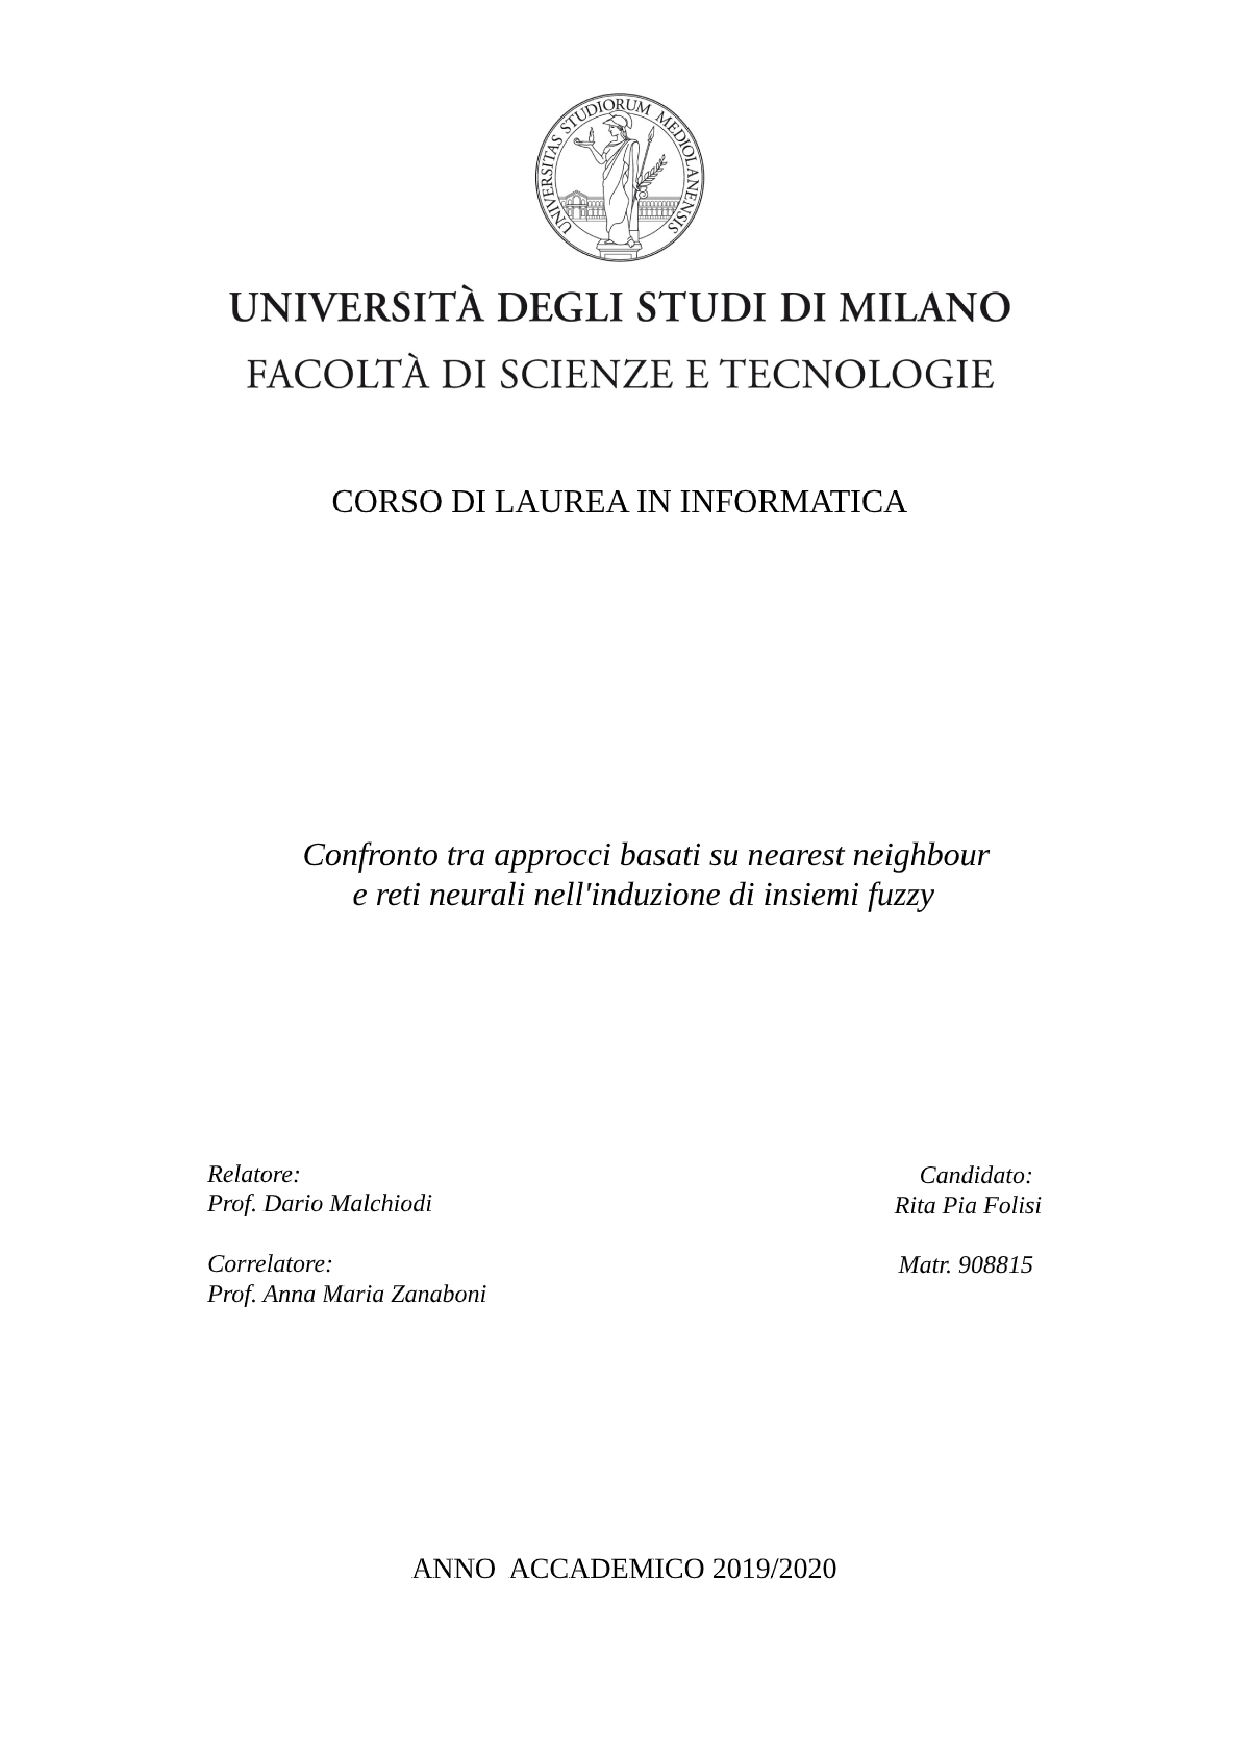
\includepdf{Frontespizio.pdf}
    \thispagestyle{empty}
  \end{titlepage}



	\pagenumbering{arabic}

	\chapter*{Riassunto dell'elaborato}
In questo elaborato si descrive il tirocinio, effettuato presso l'Università degli Studi di Milano, che riguarda la ricerca, la modifica e il riuso di algoritmi per l'induzione della funzione di appartenenza a insiemi fuzzy. 

Nell'ambito dell'apprendimento automatico, una classe di problemi che ha assunto grande rilevanza è legata alla classificazione: dato un oggetto, ci si aspetta che si riesca a predire la sua classe di appartenenza. Esistono vari approcci al problema, ognuno dei quali con i propri punti di forza e di debolezza. Nel tirocinio ci si è occupati di insiemi fuzzy, dal momento che riescono a cogliere l'ambiguità caratterizzante il linguaggio naturale, consentendo una maggiore flessibilità nella classificazione stessa. Nell'ambito degli insiemi fuzzy, fondamentale è il concetto di funzione di appartenenza, che definisce il grado con cui un dato oggetto può appartenere ad una classe. Ricoprendo valori da 0 a 1, la funzione di appartenenza riesce così a sintetizzare anche la parziale appartenenza di un oggetto ad una data classe, superando il binarismo della logica classica. 

In letteratura sono stati presentati molteplici modi per poter indurre la funzione di appartenenza. Nel tirocinio sono stati esaminati algoritmi basati sulle reti neurali e sul k-Nearest Neighbor, illustrandone inoltre le principali varianti. In particolare, è stato implementato un algoritmo per ogni famiglia: per le reti neurali ci si è soffermati sul Fuzzy min-max Neural Network, mentre per il k-Nearest Neighbor è stato analizzato il Fuzzy k-Nearest Neighbor. Per entrambi gli algoritmi si è partiti da codice preesistente sul quale sono state attuate modifiche per poter in seguito effettuare esperimenti e valutare le prestazioni. Gli algoritmi sono stati valutati sui dataset Iris e Breast-Cancer, ottenendo dei buoni risultati. Il Fuzzy min-max classifica i dati con un'accuratezza maggiore e impiega meno tempo a elaborarli e a effettuare predizioni; il Fuzzy k-Nearest Neighbor, invece, fornisce un errore minore nell'indurre i gradi di appartenenza. 

L'elaborato è strutturato come segue: nel Capitolo 1 sono introdotte le tematiche relative all'apprendimento automatico e logica fuzzy, illustrando il problema sul quale l'elaborato si concentra. Nel Capitolo 2 si passano in rassegna i concetti di reti neurali e di k-Nearest Neighbor, per illustrarne il funzionamento e fornire una panoramica delle possibili varianti. Nel Capitolo 3 viene infine descritta l'implementazione e si forniscono i risultati degli esperimenti effettuati, sotto forma di tabelle e grafici. 

\end{document}